
%% bare_conf.tex
%% V1.4b
%% 2015/08/26
%% by Michael Shell
%% See:
%% http://www.michaelshell.org/
%% for current contact information.
%%
%% This is a skeleton file demonstrating the use of IEEEtran.cls
%% (requires IEEEtran.cls version 1.8b or later) with an IEEE
%% conference paper.
%%
%% Support sites:
%% http://www.michaelshell.org/tex/ieeetran/
%% http://www.ctan.org/pkg/ieeetran
%% and
%% http://www.ieee.org/

%%*************************************************************************
%% Legal Notice:
%% This code is offered as-is without any warranty either expressed or
%% implied; without even the implied warranty of MERCHANTABILITY or
%% FITNESS FOR A PARTICULAR PURPOSE! 
%% User assumes all risk.
%% In no event shall the IEEE or any contributor to this code be liable for
%% any damages or losses, including, but not limited to, incidental,
%% consequential, or any other damages, resulting from the use or misuse
%% of any information contained here.
%%
%% All comments are the opinions of their respective authors and are not
%% necessarily endorsed by the IEEE.
%%
%% This work is distributed under the LaTeX Project Public License (LPPL)
%% ( http://www.latex-project.org/ ) version 1.3, and may be freely used,
%% distributed and modified. A copy of the LPPL, version 1.3, is included
%% in the base LaTeX documentation of all distributions of LaTeX released
%% 2003/12/01 or later.
%% Retain all contribution notices and credits.
%% ** Modified files should be clearly indicated as such, including  **
%% ** renaming them and changing author support contact information. **
%%*************************************************************************


% *** Authors should verify (and, if needed, correct) their LaTeX system  ***
% *** with the testflow diagnostic prior to trusting their LaTeX platform ***
% *** with production work. The IEEE's font choices and paper sizes can   ***
% *** trigger bugs that do not appear when using other class files.       ***                          ***
% The testflow support page is at:
% http://www.michaelshell.org/tex/testflow/



\documentclass[conference]{IEEEtran}
% Some Computer Society conferences also require the compsoc mode option,
% but others use the standard conference format.
%
% If IEEEtran.cls has not been installed into the LaTeX system files,
% manually specify the path to it like:
% \documentclass[conference]{../sty/IEEEtran}





% Some very useful LaTeX packages include:
% (uncomment the ones you want to load)


% *** MISC UTILITY PACKAGES ***
\usepackage[pdftex]{graphicx}
\usepackage{subfig}
\usepackage{lipsum}% http://ctan.org/pkg/lipsum
\usepackage{multicol}% http://ctan.org/pkg/multicols
%
%\usepackage{ifpdf}
% Heiko Oberdiek's ifpdf.sty is very useful if you need conditional
% compilation based on whether the output is pdf or dvi.
% usage:
% \ifpdf
%   % pdf code
% \else
%   % dvi code
% \fi
% The latest version of ifpdf.sty can be obtained from:
% http://www.ctan.org/pkg/ifpdf
% Also, note that IEEEtran.cls V1.7 and later provides a builtin
% \ifCLASSINFOpdf conditional that works the same way.
% When switching from latex to pdflatex and vice-versa, the compiler may
% have to be run twice to clear warning/error messages.






% *** CITATION PACKAGES ***
%
\usepackage{cite}
%\usepackage[counterclockwise, figuresleft]{rotating}
% cite.sty was written by Donald Arseneau
% V1.6 and later of IEEEtran pre-defines the format of the cite.sty package
% \cite{} output to follow that of the IEEE. Loading the cite package will
% result in citation numbers being automatically sorted and properly
% "compressed/ranged". e.g., [1], [9], [2], [7], [5], [6] without using
% cite.sty will become [1], [2], [5]--[7], [9] using cite.sty. cite.sty's
% \cite will automatically add leading space, if needed. Use cite.sty's
% noadjust option (cite.sty V3.8 and later) if you want to turn this off
% such as if a citation ever needs to be enclosed in parenthesis.
% cite.sty is already installed on most LaTeX systems. Be sure and use
% version 5.0 (2009-03-20) and later if using hyperref.sty.
% The latest version can be obtained at:
% http://www.ctan.org/pkg/cite
% The documentation is contained in the cite.sty file itself.






% *** GRAPHICS RELATED PACKAGES ***
%
\ifCLASSINFOpdf
  % \usepackage[pdftex]{graphicx}
  % declare the path(s) where your graphic files are
  % \graphicspath{{../pdf/}{../jpeg/}}
  % and their extensions so you won't have to specify these with
  % every instance of \includegraphics
  % \DeclareGraphicsExtensions{.pdf,.jpeg,.png}
\else
  % or other class option (dvipsone, dvipdf, if not using dvips). graphicx
  % will default to the driver specified in the system graphics.cfg if no
  % driver is specified.
  % \usepackage[dvips]{graphicx}
  % declare the path(s) where your graphic files are
  % \graphicspath{{../eps/}}
  % and their extensions so you won't have to specify these with
  % every instance of \includegraphics
  % \DeclareGraphicsExtensions{.eps}
\fi
% graphicx was written by David Carlisle and Sebastian Rahtz. It is
% required if you want graphics, photos, etc. graphicx.sty is already
% installed on most LaTeX systems. The latest version and documentation
% can be obtained at: 
% http://www.ctan.org/pkg/graphicx
% Another good source of documentation is "Using Imported Graphics in
% LaTeX2e" by Keith Reckdahl which can be found at:
% http://www.ctan.org/pkg/epslatex
%
% latex, and pdflatex in dvi mode, support graphics in encapsulated
% postscript (.eps) format. pdflatex in pdf mode supports graphics
% in .pdf, .jpeg, .png and .mps (metapost) formats. Users should ensure
% that all non-photo figures use a vector format (.eps, .pdf, .mps) and
% not a bitmapped formats (.jpeg, .png). The IEEE frowns on bitmapped formats
% which can result in "jaggedy"/blurry rendering of lines and letters as
% well as large increases in file sizes.
%
% You can find documentation about the pdfTeX application at:
% http://www.tug.org/applications/pdftex





% *** MATH PACKAGES ***
%
%\usepackage{amsmath}
% A popular package from the American Mathematical Society that provides
% many useful and powerful commands for dealing with mathematics.
%
% Note that the amsmath package sets \interdisplaylinepenalty to 10000
% thus preventing page breaks from occurring within multiline equations. Use:
%\interdisplaylinepenalty=2500
% after loading amsmath to restore such page breaks as IEEEtran.cls normally
% does. amsmath.sty is already installed on most LaTeX systems. The latest
% version and documentation can be obtained at:
% http://www.ctan.org/pkg/amsmath





% *** SPECIALIZED LIST PACKAGES ***
%
%\usepackage{algorithmic}
% algorithmic.sty was written by Peter Williams and Rogerio Brito.
% This package provides an algorithmic environment fo describing algorithms.
% You can use the algorithmic environment in-text or within a figure
% environment to provide for a floating algorithm. Do NOT use the algorithm
% floating environment provided by algorithm.sty (by the same authors) or
% algorithm2e.sty (by Christophe Fiorio) as the IEEE does not use dedicated
% algorithm float types and packages that provide these will not provide
% correct IEEE style captions. The latest version and documentation of
% algorithmic.sty can be obtained at:
% http://www.ctan.org/pkg/algorithms
% Also of interest may be the (relatively newer and more customizable)
% algorithmicx.sty package by Szasz Janos:
% http://www.ctan.org/pkg/algorithmicx




% *** ALIGNMENT PACKAGES ***
%
%\usepackage{array}
% Frank Mittelbach's and David Carlisle's array.sty patches and improves
% the standard LaTeX2e array and tabular environments to provide better
% appearance and additional user controls. As the default LaTeX2e table
% generation code is lacking to the point of almost being broken with
% respect to the quality of the end results, all users are strongly
% advised to use an enhanced (at the very least that provided by array.sty)
% set of table tools. array.sty is already installed on most systems. The
% latest version and documentation can be obtained at:
% http://www.ctan.org/pkg/array


% IEEEtran contains the IEEEeqnarray family of commands that can be used to
% generate multiline equations as well as matrices, tables, etc., of high
% quality.




% *** SUBFIGURE PACKAGES ***
%\ifCLASSOPTIONcompsoc
%  \usepackage[caption=false,font=normalsize,labelfont=sf,textfont=sf]{subfig}
%\else
%  \usepackage[caption=false,font=footnotesize]{subfig}
%\fi
% subfig.sty, written by Steven Douglas Cochran, is the modern replacement
% for subfigure.sty, the latter of which is no longer maintained and is
% incompatible with some LaTeX packages including fixltx2e. However,
% subfig.sty requires and automatically loads Axel Sommerfeldt's caption.sty
% which will override IEEEtran.cls' handling of captions and this will result
% in non-IEEE style figure/table captions. To prevent this problem, be sure
% and invoke subfig.sty's "caption=false" package option (available since
% subfig.sty version 1.3, 2005/06/28) as this is will preserve IEEEtran.cls
% handling of captions.
% Note that the Computer Society format requires a larger sans serif font
% than the serif footnote size font used in traditional IEEE formatting
% and thus the need to invoke different subfig.sty package options depending
% on whether compsoc mode has been enabled.
%
% The latest version and documentation of subfig.sty can be obtained at:
% http://www.ctan.org/pkg/subfig




% *** FLOAT PACKAGES ***
%
%\usepackage{fixltx2e}
% fixltx2e, the successor to the earlier fix2col.sty, was written by
% Frank Mittelbach and David Carlisle. This package corrects a few problems
% in the LaTeX2e kernel, the most notable of which is that in current
% LaTeX2e releases, the ordering of single and double column floats is not
% guaranteed to be preserved. Thus, an unpatched LaTeX2e can allow a
% single column figure to be placed prior to an earlier double column
% figure.
% Be aware that LaTeX2e kernels dated 2015 and later have fixltx2e.sty's
% corrections already built into the system in which case a warning will
% be issued if an attempt is made to load fixltx2e.sty as it is no longer
% needed.
% The latest version and documentation can be found at:
% http://www.ctan.org/pkg/fixltx2e


%\usepackage{stfloats}
% stfloats.sty was written by Sigitas Tolusis. This package gives LaTeX2e
% the ability to do double column floats at the bottom of the page as well
% as the top. (e.g., "\begin{figure*}[!b]" is not normally possible in
% LaTeX2e). It also provides a command:
%\fnbelowfloat
% to enable the placement of footnotes below bottom floats (the standard
% LaTeX2e kernel puts them above bottom floats). This is an invasive package
% which rewrites many portions of the LaTeX2e float routines. It may not work
% with other packages that modify the LaTeX2e float routines. The latest
% version and documentation can be obtained at:
% http://www.ctan.org/pkg/stfloats
% Do not use the stfloats baselinefloat ability as the IEEE does not allow
% \baselineskip to stretch. Authors submitting work to the IEEE should note
% that the IEEE rarely uses double column equations and that authors should try
% to avoid such use. Do not be tempted to use the cuted.sty or midfloat.sty
% packages (also by Sigitas Tolusis) as the IEEE does not format its papers in
% such ways.
% Do not attempt to use stfloats with fixltx2e as they are incompatible.
% Instead, use Morten Hogholm'a dblfloatfix which combines the features
% of both fixltx2e and stfloats:
%
% \usepackage{dblfloatfix}
% The latest version can be found at:
% http://www.ctan.org/pkg/dblfloatfix




% *** PDF, URL AND HYPERLINK PACKAGES ***
%
%\usepackage{url}
% url.sty was written by Donald Arseneau. It provides better support for
% handling and breaking URLs. url.sty is already installed on most LaTeX
% systems. The latest version and documentation can be obtained at:
% http://www.ctan.org/pkg/url
% Basically, \url{my_url_here}.




% *** Do not adjust lengths that control margins, column widths, etc. ***
% *** Do not use packages that alter fonts (such as pslatex).         ***
% There should be no need to do such things with IEEEtran.cls V1.6 and later.
% (Unless specifically asked to do so by the journal or conference you plan
% to submit to, of course. )


% correct bad hyphenation here
\hyphenation{op-tical net-works semi-conduc-tor}


\begin{document}
%
% paper title
% Titles are generally capitalized except for words such as a, an, and, as,
% at, but, by, for, in, nor, of, on, or, the, to and up, which are usually
% not capitalized unless they are the first or last word of the title.
% Linebreaks \\ can be used within to get better formatting as desired.
% Do not put math or special symbols in the title.
\title{Trust in Vehicle-to-Vehicle Communication}


% author names and affiliations
% use a multiple column layout for up to three different
% affiliations
\author{\IEEEauthorblockN{Boakye Dankwa, Rajeev R. Raje, Raghavendran Vijayan, Darsh Sanghavi}
\IEEEauthorblockA{Department of Computer and Information Science\\
Indiana University Purdue University\\
Indianapolis, Indiana, USA}}
%\and
%\IEEEauthorblockN{Boakye Dankwa}
%\IEEEauthorblockA{Computer and Information Science\\
%Indiana University - Purdue University\\
%Indianapolis, Indiana 46202\\
%Email: bdankwa@iupui.edu}
%\and
%\IEEEauthorblockN{Raghavendran Vijayan\\ and Darsh Sanghavi}
%\IEEEauthorblockA{Computer and Information Science\\
%Indianapolis, Indiana 46202}}

% conference papers do not typically use \thanks and this command
% is locked out in conference mode. If really needed, such as for
% the acknowledgment of grants, issue a \IEEEoverridecommandlockouts
% after \documentclass

% for over three affiliations, or if they all won't fit within the width
% of the page, use this alternative format:
% 
%\author{\IEEEauthorblockN{Michael Shell\IEEEauthorrefmark{1},
%Homer Simpson\IEEEauthorrefmark{2},
%James Kirk\IEEEauthorrefmark{3}, 
%Montgomery Scott\IEEEauthorrefmark{3} and
%Eldon Tyrell\IEEEauthorrefmark{4}}
%\IEEEauthorblockA{\IEEEauthorrefmark{1}School of Electrical and Computer Engineering\\
%Georgia Institute of Technology,
%Atlanta, Georgia 30332--0250\\ Email: see http://www.michaelshell.org/contact.html}
%\IEEEauthorblockA{\IEEEauthorrefmark{2}Twentieth Century Fox, Springfield, USA\\
%Email: homer@thesimpsons.com}
%\IEEEauthorblockA{\IEEEauthorrefmark{3}Starfleet Academy, San Francisco, California 96678-2391\\
%Telephone: (800) 555--1212, Fax: (888) 555--1212}
%\IEEEauthorblockA{\IEEEauthorrefmark{4}Tyrell Inc., 123 Replicant Street, Los Angeles, California 90210--4321}}




% use for special paper notices
%\IEEEspecialpapernotice{(Invited Paper)}




% make the title area
\maketitle

% As a general rule, do not put math, special symbols or citations
% in the abstract
\begin{abstract}
In traditional Pedestrian Automatic Emergency Braking (PAEB) system, vehicles equipped with onboard sensors such as (rader, camera, and infrared) detects pedestrians, alerts the driver and/ or automatically take action to prevent vehicle-pedestrian collision. In some situations, a vehicle may not be able to detect a pedestrian due to  blind spots. Such a vehicle could benefit from the sensor data from neighboring vehicles in making such safety critical decisions. We propose a trust model for ensuring shared data are valid and trustworthy for use in making safety critical decisions. Simulation results of the proposed trust model show promise.
\end{abstract}

\begin{IEEEkeywords}
TODO; TODO; TODO; 

\end{IEEEkeywords}




% For peer review papers, you can put extra information on the cover
% page as needed:
% \ifCLASSOPTIONpeerreview
% \begin{center} \bfseries EDICS Category: 3-BBND \end{center}
% \fi
%
% For peerreview papers, this IEEEtran command inserts a page break and
% creates the second title. It will be ignored for other modes.
\IEEEpeerreviewmaketitle



\section{Introduction}
% no \IEEEPARstart
In traditional Pedestrian Automatic Emergency Braking (PAEB) system, vehicles equipped with onboard sensors such as (rader, camera, and infrared) detects pedestrians, alerts the driver and/ or automatically takes action to prevent vehicle-pedestrian collision. In some situations such as shown in Figure \ref{obstc}, the sensors of the black sedan may not detect the pedestrian which could result in a crash. However, if the vehicles in the scenario shared sensor information in a  vehicle-to-vehicle (V2V) communication fashion, such a crash can be avoided.

\begin{figure}[h]
\centering
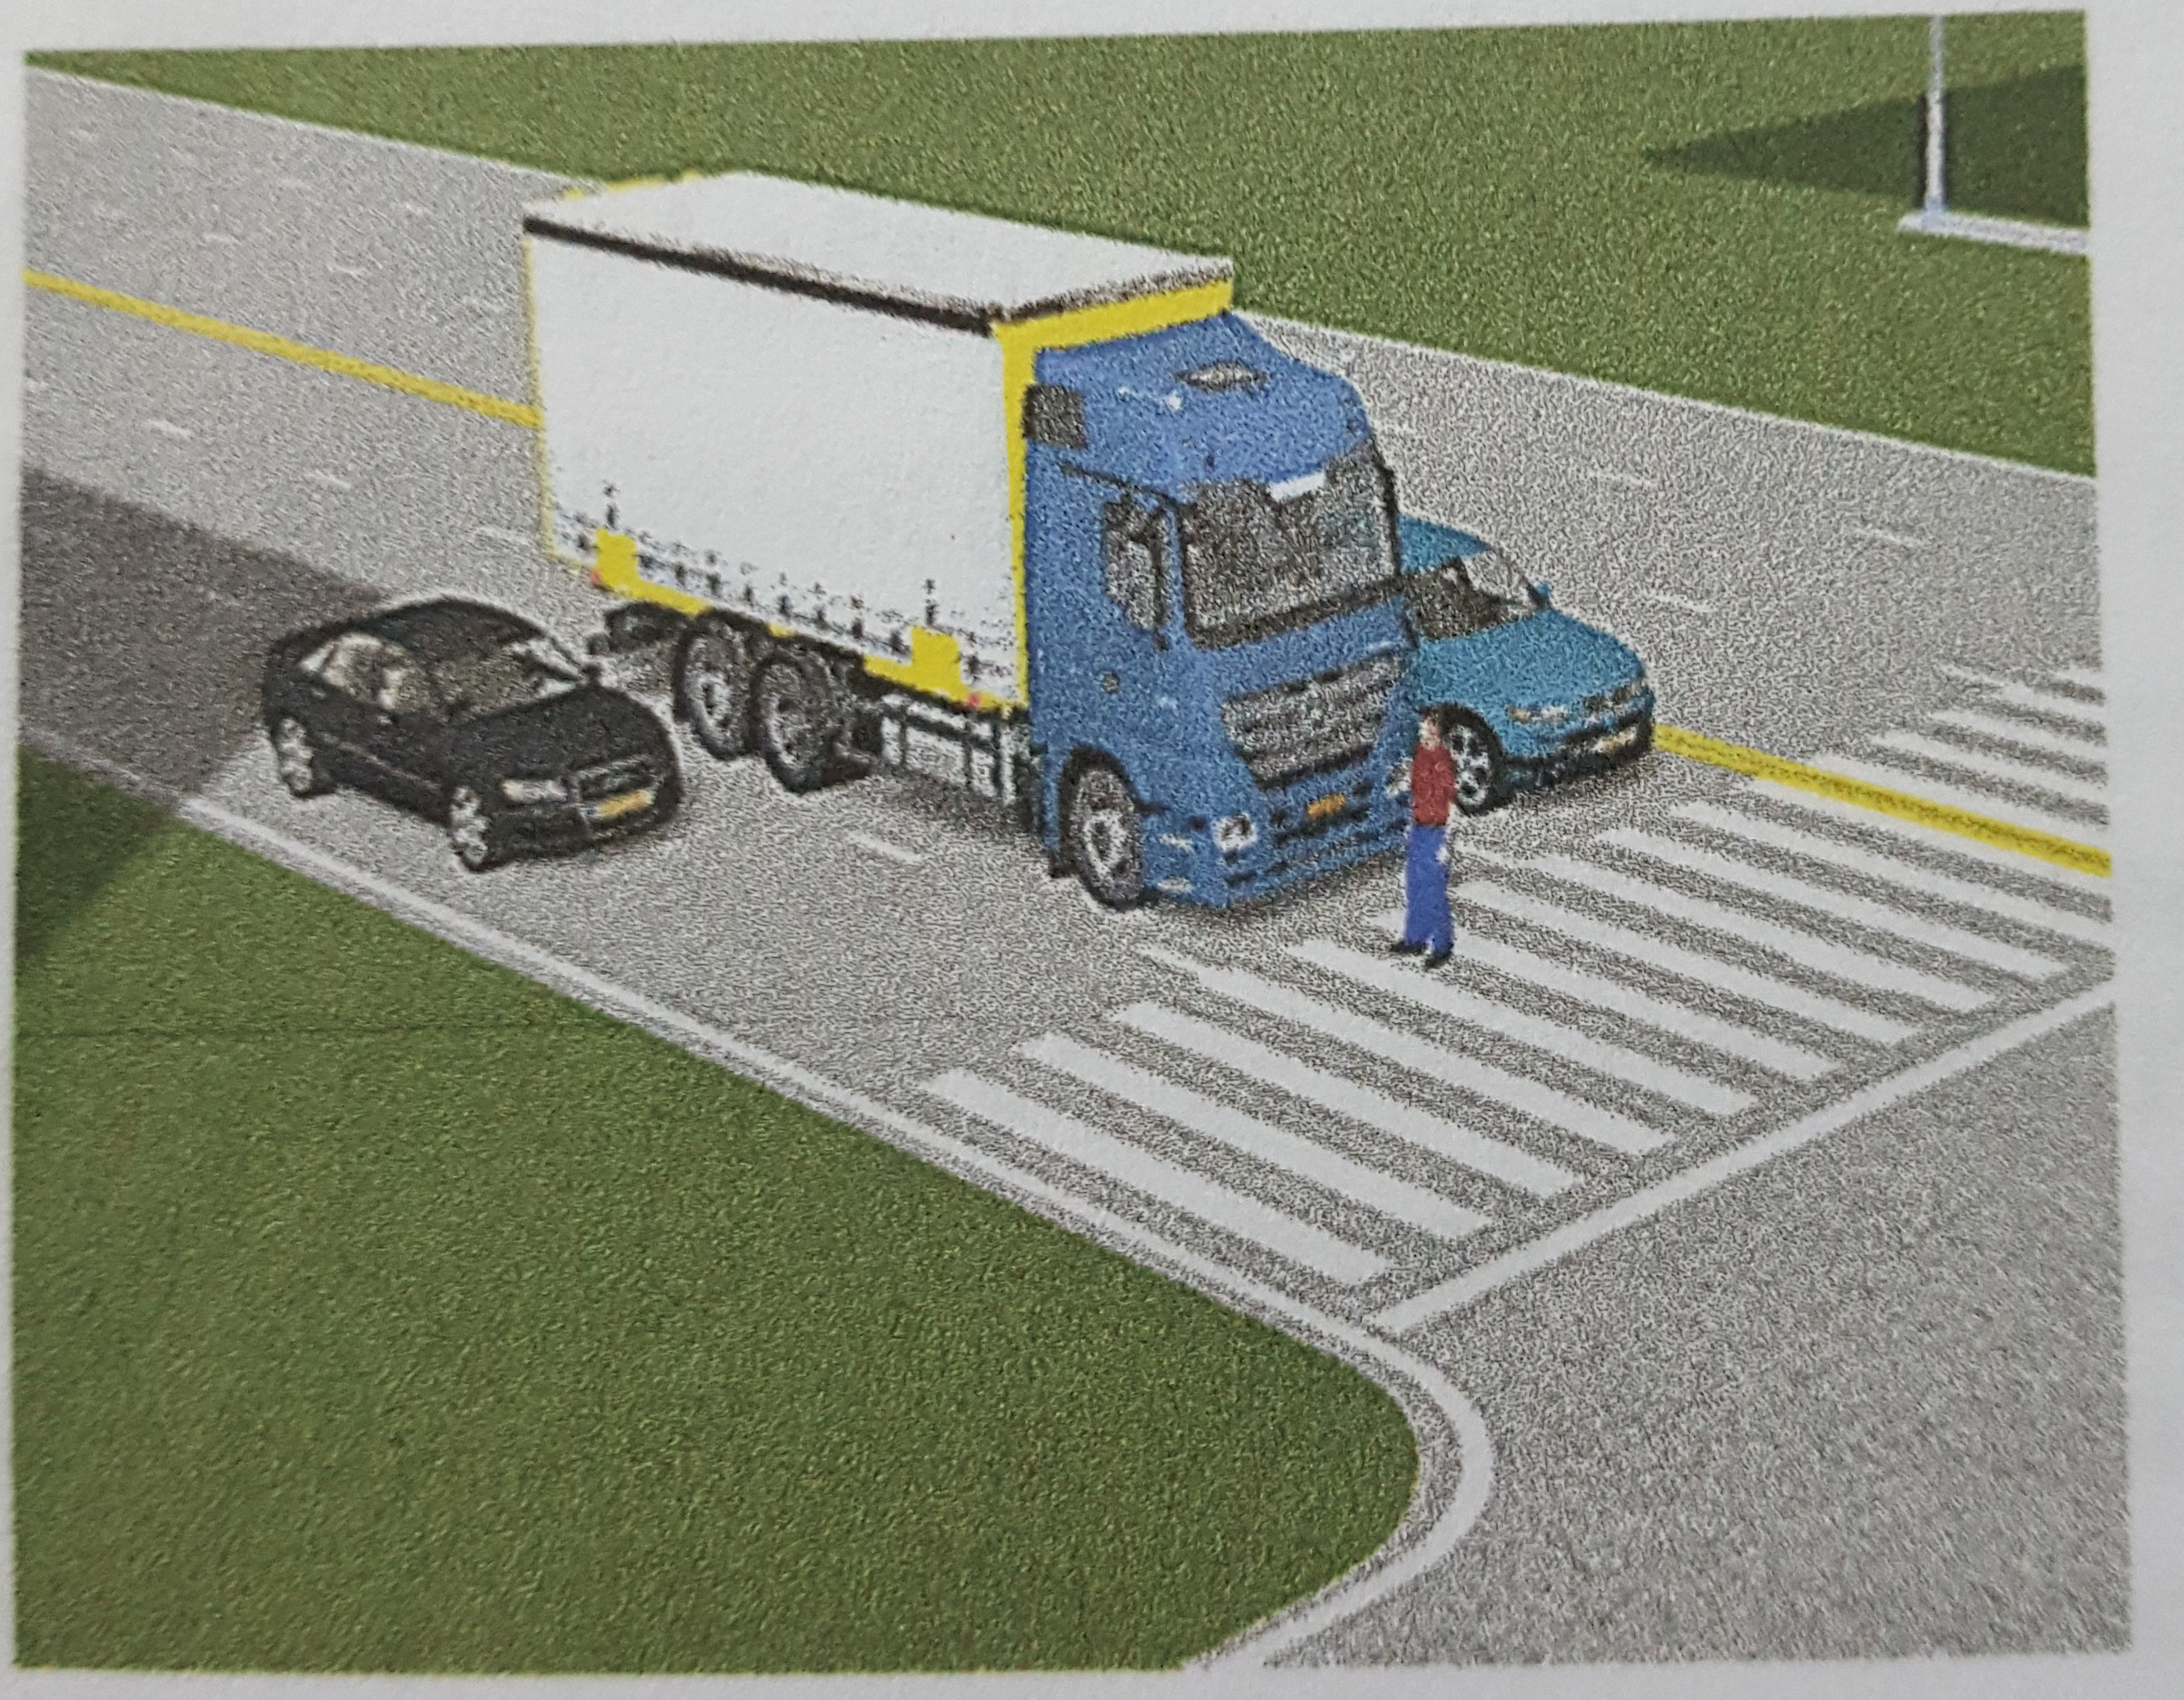
\includegraphics[width=3.5in]{V2VPAEB_Scenario.png}
\caption{Crash Scenario due to an obstruction in the middle}
\label{obstc}
\end{figure}

In V2V communication, every transceiver device involved sends data such as pedestrian cross, toll gate, accidents and so to other transceiver device. Constraints such as network QoS, quality of vehicle sensors and systems directly impact the quality of the exchanged data. These messages are used in making critical decisions such as slowing down to avoid collision with a pedestrian. As such, the validity of these messages play an important role in making safety critical decision. For example, are the messages referring to the same pedestrian, or are they referring to an object by the roadside.

Trust is crucial if such messages are to be used to improve the performance of a PAEB system. For example, imminent vehicle – pedestrian collision can be avoided in a vehicle which cannot directly sense the pedestrian and therefore must rely on messages received from neighboring vehicles.

We attempt to contribute to the area of V2V-PAEB research by focusing on trust in the system. We propose a trust model to quantify trust for communications in a V2V-PAEB system. Our model filters incoming messages, evaluate trustworthiness and forwards the messages, along with their quantified trust data, for safety decision to be made upstream. Our trust model will seamlessly integrate with the Transportation Active Safety Institute (TASI) computer simulation at IUPUI TASI lab. Communications between the vehicles can be secured with appropriate authentication and encryption technologies, therefore we assume secure communication channels between vehicles.
%\hfill mds
 
%\hfill August 26, 2015
\section{Related Work} \label{lreview}
Trust is a subjective concept, it's a relationship existing between two participants. \cite{trustSurvey2015} defines trust as:
\newline
\newline
"Trust is the willingness of the trustor (evaluator) to take risk on a subjective belief that a trustee (evaluatee) will exhibit reliable behavior to maximize the trustor’s interest under uncertainty (e.g. ambiguity due to conflicting evidence and /or ignorance caused by complete lack of evidence) of a given situation based on the cognitive assessment of past experience with the trustee"
\newline
\newline
For example, in human associations, we trust other people based on our past experiences with them and we are able to rely on such experiences to believe that they will exhibit reliable behavior in unfamiliar or ambiguous situations. On the contrary, if we distrust someone, then we believe we can not assume they will exhibit reliable behavior under such conditions. It is important to note that trust is contextual and constantly evolving. For example, a trusted person can exhibit reliable behavior in one scenario but unreliable behavior in a different contest (trusting Bob as a good math teacher, but a bad basketball player). Also if you have trusted Alice with your credit card and you end up with unknown charges, your trust for her with respect to this context will reduce. It is in this notion that we propose a trust model for the V2V application.

Trust management system is the framework designed to help make better decisions based on trust information. Trust management system consists of three components: trust modeling, trust inference and trust decision, and the applicable context \cite{artIntel2005}. See Figure \ref{tmanagement}.

\begin{figure}[h]
\centering
\includegraphics[width=3.5in]{Trust_Management_System.png}
\caption{Trust Management System}
\label{tmanagement}
\end{figure}

This deals with how to represent trust in computational models using available raw data. Trust can either be numerical or categorical. Discrete and continuous numerical values are usually used to quantitatively measure trust \cite{trustSurvey2015}.

Sometimes there is the need to aggregate trust from various participants in order to infer trust between two parties. There are two important operators in trust reference schemes: concatenation operator and aggregation operator \cite{trustAggreg06}. Transitivity operator is used to calculate trust propagation in a single chain. Aggregation operator is used for combining parallel trust paths between the truster and the trustee in the case where there exist more than one trust path between them \cite{logicUnProb2001}.

The last component of the trust model is decision making. This is where a decision is made based on the evaluated trust between the truster and the trustee.

\section{Proposed Trust Management System for V2V-PAEB} \label{contribution}
We model trust as a continuous numerical value in the range [0 1]. Zero (0) represents complete distrust and one (1) represents complete trust. We compute a trust value for each sensor data received in messages from neighboring vehicles. Each message contain one or more sensor data. There are three trust components involved, we call these, \textit{measured trust},  \textit{short-term reputation} and \textit{long-term reputation}. These three components are then aggregated to achieve the resultant trust between a vehicle’s sensor and the V2V-PAEB decision logic. Figure \ref{tforV2V} shows the data flow relationship between our trust model and the V2V-PAEB simulation environment.

%\begin{sidewaysfigure}
%\begin{figure}[h]
%\centering
%\includegraphics[width=8.5in]{V2V_Tust_Management_System.png}
%\caption{TASI V2V-PAEB Simulation System with Trust Management}
%\label{tforV2V}
%\end{figure}
%\end{sidewaysfigure}

\begin{figure*}
  \includegraphics[width=\textwidth]{V2V_Tust_Management_System.png}
  \caption{TASI V2V-PAEB Simulation System with Trust Management}
  \label{tforV2V}
\end{figure*}

%\begin{figure}[h]
%\centering
%\includegraphics[width=6.5in]{V2V_Tust_Management_System.png}
%\caption{TASI V2V-PAEB Simulation System with Trust Management}
%\label{tforV2V}
%\end{figure}

\begin{figure}[h]
\centering
\includegraphics[width=3.5in]{Trust_Model.png}
\caption{Trust Model for TASI V2V-PAEB Simulation}
\label{tmodel}
\end{figure}

\subsubsection{Measured Trust}
We compute this trust value in two parts, first a value based on a known sensor profile, and then a value based on the error probability in the measured raw data. This model is contextual and dependent on the type of sensor and quantity being measured. For example, a typical profile for a sensor that measures a pedestrian location would include reasonable lower and upper limits in the measured value. A lower limit can be selected as zero feet from the subject vehicle in the same plane as the direction of travel. An upper limit can also be selected as some foot (based on the speed of the subject vehicle) in the same plane as the direction of travel. A value outside this range, for example, position data which indicates a pedestrian above or below the plane of travel would indicate a failed sensor and hence be deemed untrustworthy and therefore not considered in making control decisions. In a rare situation where all messages are declared failed, it will be up to the V2V-PAEB control logic to decide what safety action to take. Each sensor can have as many profiles as can be constructed. The other part of the measured trust is based on measurement error in the physical quantity. Error probability models can be used to estimate the error involved in measurements. The results of these analysis can then be mapped onto a trust plane.

\subsubsection{Short Term Reputation}
Here we maintain a local historical trust value for each vehicle we receive messages from. If a message is not received from a given vehicle after some predefined time, for example if it is no longer within range, it is dropped from this historical list. Each trust value is based on short-term history of decisions made by the V2V-PAEB control logic. This requires feedback from the V2V-PAEB control logic. For this to be feasible, the V2V-PAEB control system must be able to perform an inverse operation to map the output decision back onto the contributing vehicles. This inverse operation is problematic since the consequence of the control decision is binary (collision, no collision). Therefore we adopted a simpler universal approach where the short-term trust values of all involving vehicles are penalized (i.e. assigned a default reset value) when a collision results from a control decision. On the other hand, when collision is avoided, all involving vehicles are rewarded with a boost in their short-term trust values (i.e. trust values incremented by a fixed amount). This trust component is periodically uploaded remotely to update a long-term reputation.

\subsubsection{Long Term Reputation}
This is a historical accumulation of short-term reputation for all vehicle types. This data is maintained remotely and accessed by V2V-PAEB enabled vehicles for trust computations.

\subsubsection{Trust Aggregation}
The three trust components are then aggregated to provide a single trust value for each sensor value used for decision making. We adopted a simple weighted additive aggregation scheme.

\section{Implementation Details}
%Due to scheduling and availability of the TASI simulation team, we did not get the opportunity to integrate into the TASI simulation environment to experimentally demonstrate the performance of our trust model. Nevertheless, a simple Simulink model was developed to demonstrate how trust will be computed and will evolve in the system.

%\begin{figure}[h]
%\centering
%\includegraphics[width=6.5in]{simulink.png}
%\caption{Simulink Implementation of Trust Model}
%\label{simulink}
%\end{figure}

%Figure \ref{simulink} shows the top level Simulink model. It shows three transformed signals representing sensor data from three vehicles. Random noise is added to a component of each of the three signals to simulate error in the sensor data. The signals feed into the \textit{measured trust} model which has a predefined sensor profile and error analysis used in calculating trust values for each sensor.

For simplicity, a single sensor is considered for demonstration purposes (In a real-world application, there would be multiple sensors and therefore multiple profiles would be required). A simple range-check is used as a profile for the sensor. That is, the euclidean norm of each sensor value must fall withing a certain reasonable range to be deemed trust-worthy. When a sensor values falls outside the acceptable range, it is marked as untrustworthy and automatically assigned a trust value of 0. When a signal falls within the profile, it moves on to the error analysis. Here, we used the euclidean distance from the mean of the signals as an error measure. That is, the farther away from the mean, the less trust we assign to the signal, the closer it is, the more we trust the signal. We assign a trust value of 1 to the mean, and 0.5 to the signal farthest away from the mean. Note that 0.5 is the default trust assigned to each signal that falls within the profile. We linearly interpolate any trust values in-between these two limits.

A short term reputation model models the interaction between the output of the V2V-PAEB simulation and the trust model. If a control decision doesn't result in a vehicle-pedestrian collision, the trust value for all vehicles involved is increased by a small value (0.1). If a collision resulted from a control decision, all vehicles get a default trust value (0).

A fixed trust value of 0.5 was assigned as long-term reputation trust value for all messages. A more complex long-term reputation model will be implemented as a future extension.

The trust values from all there models are weighted and aggregated into a single trust value to be sent to the V2V-PAEB simulation control model.

\section{Results and Discussions}
The simulation consists of messages from three vehicles. For demonstration purposes, only a single sensor type was used. This could be say, the position of velocity of a pedestrian as measured by each vehicle. The signals used in the trust analysis are assumed to have been transformed to a common reference by the TASI simulation environment downstream of the trust model as shown in Figure \ref{tforV2V}. 

%\begin{figure}[h]
%\centering
%\includegraphics[width=4.5in]{Signal_norminal.png}
%\caption{Raw Sensor Signals from Neighboring Vehicles }
%\label{raw}
%\end{figure}

Figure \ref{tnormal} shows the nominal case where each of the messages fall within profile. This results in an aggregate trust profile which shows convergence of trust values for all three messages. It clearly shows that the trust for all in-profile messages converges after a few seconds.

For an out-of-profile signal such us the message from vehicle 2, the aggregate trust for vehicle 2 drops to zero (distrust) as soon as it falls out of the profile as shown in \ref{toutprofile}. The trust then gradually builds up until it eventually settles. This is an expected behavior since we have to be cautious not to trust a sensor immediately after it returns from an out-of-profile error.

The final result is how the aggregate trust of an in-profile message would behave after a collision event. Figure \ref{tcollision} shows that the aggregate trust for all messages falls to a value based on a default computed trust, the short-term reputation and long-term reputation. 

\begin{figure}[h]
\centering
\includegraphics[width=3.5in]{trust_norminal.png}
\caption{Trust for all in-profile messages}
\label{tnormal}
\end{figure}

\begin{figure}[h]
\centering
\includegraphics[width=3.5in]{trust_outside_profile.png}
\caption{Trust for out-of-profile message}
\label{toutprofile}
\end{figure}

\begin{figure}[h]
\centering
\includegraphics[width=3.5in]{trust_collision.png}
\caption{Aggregate trust after a collision event}
\label{tcollision}
\end{figure}



%\begin{figure}
%\centering
%\begin{tabular}{cc}
%\subfloat[A profile check - in-profile messages ]{\includegraphics[width = 2.8in]{Signal_profile_inrange.png}} &
%\subfloat[Trust for all in-profile messages]{\includegraphics[width = 2.8in]{trust_norminal.png}} \\
%\subfloat[A profile check - one message out of profile]{\includegraphics[width = 2.8in]{Signal_profile_outrange.png}} &
%\subfloat[Trust for out-of-profile message]{\includegraphics[width = 2.8in]{trust_outside_profile.png}} \\
%\subfloat[In-profile messages for collision scenario]{\includegraphics[width = 2.8in]{Signal_profile_inrange.png}} &
%\subfloat[Aggregate trust after a collision event]{\includegraphics[width = 2.8in]{trust_collision.png}}
%\end{tabular}
%\caption{Aggregate trust for in-profile and out-profile messages}
%\label{trust}
%\end{figure} 

%\begin{figure}[h]
%\centering
%\includegraphics[width=1.5in]{trust_collision.png}
%\caption{Aggregate trust after a collision event }
%\label{collision}
%\end{figure}
\section{Conclusions and Future Extensions}
We have proposed a trust model which estimates trust in V2V-PAEB communications. Sensor profiles are used to screen messages from inclusion in safety decisions. Error probability models are used to estimate signal error and assign trust accordingly (\textit{measured trust}), which is aggregated with a \textit{short-term reputation} and \textit{long-term reputation} to get an aggregate trust for use in V2V-PAEB control logic.

This work is an early attempt to solving the trust problem in V2V-PAEB communications. In the near future, integrating this model with the TASI simulation environment would be helpful in determining the performance of this model. Future work would involve more refinements like putting these ideas in rigorous mathematical footing. Coming up with what the \textit{long-term reputation} model would look like is also something to be worked on.

Due to the nature of this project, trust is the only concept of distributed system demonstrated in this project. We have demonstrated that trust can be infused in a V2V-PAEB system to improve vehicle-pedestrian collision avoidance. 
 
\section{Section 3} \label{section3}

%Remove this citation -->\cite{csaguidev3} 



%\cite{introDetectSvey},

 
 
 


% An example of a floating figure using the graphicx package.
% Note that \label must occur AFTER (or within) \caption.
% For figures, \caption should occur after the \includegraphics.
% Note that IEEEtran v1.7 and later has special internal code that
% is designed to preserve the operation of \label within \caption
% even when the captionsoff option is in effect. However, because
% of issues like this, it may be the safest practice to put all your
% \label just after \caption rather than within \caption{}.
%
% Reminder: the "draftcls" or "draftclsnofoot", not "draft", class
% option should be used if it is desired that the figures are to be
% displayed while in draft mode.
%
%\begin{figure}[!t]
%\centering
%\includegraphics[width=2.5in]{myfigure}
% where an .eps filename suffix will be assumed under latex, 
% and a .pdf suffix will be assumed for pdflatex; or what has been declared
% via \DeclareGraphicsExtensions.
%\caption{Simulation results for the network.}
%\label{fig_sim}
%\end{figure}

% Note that the IEEE typically puts floats only at the top, even when this
% results in a large percentage of a column being occupied by floats.


% An example of a double column floating figure using two subfigures.
% (The subfig.sty package must be loaded for this to work.)
% The subfigure \label commands are set within each subfloat command,
% and the \label for the overall figure must come after \caption.
% \hfil is used as a separator to get equal spacing.
% Watch out that the combined width of all the subfigures on a 
% line do not exceed the text width or a line break will occur.
%
%\begin{figure*}[!t]
%\centering
%\subfloat[Case I]{\includegraphics[width=2.5in]{box}%
%\label{fig_first_case}}
%\hfil
%\subfloat[Case II]{\includegraphics[width=2.5in]{box}%
%\label{fig_second_case}}
%\caption{Simulation results for the network.}
%\label{fig_sim}
%\end{figure*}
%
% Note that often IEEE papers with subfigures do not employ subfigure
% captions (using the optional argument to \subfloat[]), but instead will
% reference/describe all of them (a), (b), etc., within the main caption.
% Be aware that for subfig.sty to generate the (a), (b), etc., subfigure
% labels, the optional argument to \subfloat must be present. If a
% subcaption is not desired, just leave its contents blank,
% e.g., \subfloat[].


% An example of a floating table. Note that, for IEEE style tables, the
% \caption command should come BEFORE the table and, given that table
% captions serve much like titles, are usually capitalized except for words
% such as a, an, and, as, at, but, by, for, in, nor, of, on, or, the, to
% and up, which are usually not capitalized unless they are the first or
% last word of the caption. Table text will default to \footnotesize as
% the IEEE normally uses this smaller font for tables.
% The \label must come after \caption as always.
%
%\begin{table}[!t]
%% increase table row spacing, adjust to taste
%\renewcommand{\arraystretch}{1.3}
% if using array.sty, it might be a good idea to tweak the value of
% \extrarowheight as needed to properly center the text within the cells
%\caption{An Example of a Table}
%\label{table_example}
%\centering
%% Some packages, such as MDW tools, offer better commands for making tables
%% than the plain LaTeX2e tabular which is used here.
%\begin{tabular}{|c||c|}
%\hline
%One & Two\\
%\hline
%Three & Four\\
%\hline
%\end{tabular}
%\end{table}


% Note that the IEEE does not put floats in the very first column
% - or typically anywhere on the first page for that matter. Also,
% in-text middle ("here") positioning is typically not used, but it
% is allowed and encouraged for Computer Society conferences (but
% not Computer Society journals). Most IEEE journals/conferences use
% top floats exclusively. 
% Note that, LaTeX2e, unlike IEEE journals/conferences, places
% footnotes above bottom floats. This can be corrected via the
% \fnbelowfloat command of the stfloats package.




\section{Conclusion} \label{conclude}


% conference papers do not normally have an appendix


% use section* for acknowledgment
%\section*{Acknowledgment}


%The authors would like to thank...





% trigger a \newpage just before the given reference
% number - used to balance the columns on the last page
% adjust value as needed - may need to be readjusted if
% the document is modified later
%\IEEEtriggeratref{8}
% The "triggered" command can be changed if desired:
%\IEEEtriggercmd{\enlargethispage{-5in}}

% references section

% can use a bibliography generated by BibTeX as a .bbl file
% BibTeX documentation can be easily obtained at:
% http://mirror.ctan.org/biblio/bibtex/contrib/doc/
% The IEEEtran BibTeX style support page is at:
% http://www.michaelshell.org/tex/ieeetran/bibtex/
\bibliographystyle{IEEEtran}
% argument is your BibTeX string definitions and bibliography database(s)
\bibliography{References}
%
% <OR> manually copy in the resultant .bbl file
% set second argument of \begin to the number of references
% (used to reserve space for the reference number labels box)
%\begin{thebibliography}{1}

%\bibitem{IEEEhowto:kopka}
%H.~Kopka and P.~W. Daly, \emph{A Guide to \LaTeX}, 3rd~ed.\hskip 1em plus
%  0.5em minus 0.4em\relax Harlow, England: Addison-Wesley, 1999.

%\end{thebibliography}

%\bibliographystyle{plain}
%\bibliography{References}


% that's all folks
\end{document}


